
%%%%%%%%%%%%%%%%%%%%%%%%%%%%%%%%%%%%%%%%%%%%%%%%%%%%%%%%%%%
% Configuration
\def\thekindofdocument{Lecture Notes}
\def\thesubtitle{Chapter 2: Time-Continuous Signals and Systems}
\def\therevision{1}
\def\therevisiondate{2020-05-11}

%%%%%%%%%%%%%%%%%%%%%%%%%%%%%%%%%%%%%%%%%%%%%%%%%%%%%%%%%%%
% Header
% SPDX-License-Identifier: CC-BY-SA-4.0
%
% Copyright (c) 2020 Philipp Le
%
% Except where otherwise noted, this work is licensed under a
% Creative Commons Attribution-ShareAlike 4.0 License.
%
% Please find the full copy of the licence at:
% https://creativecommons.org/licenses/by-sa/4.0/legalcode

\documentclass[%
	a4paper,%
	twoside,%
	%bibliography=totocnumbered,
	numbers=noenddot,%
	parskip=half,%
	headsepline,%
	footsepline,%
	headings=small,%
	12pt,%
]{scrreprt}

%%%%%%%%%%%%%%%%%%%%%%%%%%%%%%%%%%%%%%%%%%%%%%%%%%%%%%%%%%%%%%%%%%%%%%%%%%%
% Language and fonts
\usepackage[UKenglish]{babel}
\usepackage[utf8]{inputenc}
\usepackage[OT2,T1]{fontenc}
\usepackage{lmodern}
\usepackage{microtype}
\usepackage{array}

%%%%%%%%%%%%%%%%%%%%%%%%%%%%%%%%%%%%%%%%%%%%%%%%%%%%%%%%%%%%%%%%%%%%%%%%%%%
% Graphics

\usepackage{graphicx}
\usepackage{pdfpages}

% TikZ
\usepackage{tikz}
\usepackage{pgf}
\usepackage{pgfplots}
\usepackage{pgfplotstable}
\pgfplotsset{compat=newest}
\pgfplotsset{
	scriptsize/.style={
		width=4.5cm,
		height=,
		legend style={font=\scriptsize},
		tick label style={font=\scriptsize},
		label style={font=\footnotesize},
		title style={font=\footnotesize},
		every axis title shift=0pt,
		max space between ticks=15,
		every mark/.append style={mark size=7},
		major tick length=0.1cm,
		minor tick length=0.066cm,
	},
}
\pgfplotsset{legend cell align=left}
\pgfplotsset{xmajorgrids}
\pgfplotsset{ymajorgrids}
\pgfplotsset{scale only axis}
\pgfplotsset{every axis plot/.append style={line width=1pt}}
\addto\extrasngerman{\pgfplotsset{/pgf/number format/.cd,set decimal separator={{{,}}}}}
\pgfplotsset{/pgf/number format/.cd,1000 sep={\,}}
\usetikzlibrary{positioning}
\usetikzlibrary{shapes.arrows}
\usetikzlibrary{shapes,arrows}
\usetikzlibrary{decorations.pathreplacing}
\usetikzlibrary{math}
\usepackage{pgf-umlsd}

% Circuits
\usepackage[european]{circuitikz}

% Custom TikZ blocks
\tikzset{
	block/.style={
		rectangle,
		align=center,
		minimum height=1cm,
		inner sep=.5cm,
		rounded corners=.15cm
	}
}

% Colours
\usepackage{xcolor}
\usepackage{color}

% Subfigures
\usepackage{subfig}

% Controlling floats
%\renewcommand{\topfraction}{0.8}
%\renewcommand{\bottomfraction}{0.33}
%\renewcommand{\floatpagefraction}{0.66}
%\renewcommand{\textfraction}{0.10}

% Custom functions
\tikzmath{
	function sinc(\x) {
		if  abs(\x) < .001 then { % (|x| < .001) ~ (x = 0)
			return 1;
		} else {
			return sin(\x r)/\x;
		};
	};
}
\tikzmath{
	function asinc(\x, \y) {
		if  abs(\x) < .001 then { % (|x| < .001) ~ (x = 0)
			return 1;
		} else {
			return sin(\y * deg(\x) / 2)/(\y * sin(deg(\x)/2));
		};
	};
}

%%%%%%%%%%%%%%%%%%%%%%%%%%%%%%%%%%%%%%%%%%%%%%%%%%%%%%%%%%%%%%%%%%%%%%%%%%%
% Symbols

\usepackage{textcomp}

% Mathematics
\usepackage{amsmath}
\usepackage{amssymb}
\usepackage{bm}
\usepackage{trsym}

% Quotes
\usepackage{csquotes}

% Formatting units
\usepackage[load-configurations=binary]{siunitx}
\sisetup{per-mode=fraction,mode=math}
\addto\extrasngerman{\sisetup{output-decimal-marker={,}}}
\addto\extrasenglish{\sisetup{output-decimal-marker={.}}}
\addto\extrasngerman{\sisetup{range-phrase={ bis~}}} 
\addto\extrasenglish{\sisetup{range-phrase={ to~}}}

% Cyrillic
\DeclareSymbolFont{cyrletters}{OT2}{wncyr}{m}{n}
\DeclareMathSymbol{\Sha}{\mathalpha}{cyrletters}{"58}

% Custom symbols
%\newcommand{\vect}[1]{\boldsymbol{\vec{\mathbf{#1}}}}
\newcommand{\vect}[1]{\vec{\bm{#1}}}
\newcommand{\cmplxvect}[1]{\vect{\underline{#1}}}
\newcommand{\mat}[1]{\bm{\mathrm{#1}}}
\newcommand{\E}{\mathrm{E}}
\newcommand{\Var}{\mathrm{Var}}
\newcommand{\Cov}{\mathrm{Cov}}
\def\j{\mathsf{j}}

%%%%%%%%%%%%%%%%%%%%%%%%%%%%%%%%%%%%%%%%%%%%%%%%%%%%%%%%%%%%%%%%%%%%%%%%%%%
% Tables

% Lines for Tables
\usepackage{booktabs}

\usepackage{multirow}
\usepackage{longtable}

\usepackage{makecell}

%%%%%%%%%%%%%%%%%%%%%%%%%%%%%%%%%%%%%%%%%%%%%%%%%%%%%%%%%%%%%%%%%%%%%%%%%%%
% Page layout

\usepackage{setspace}
\onehalfspacing

\usepackage[a4paper, margin=2.5cm, headheight=22pt]{geometry}

\usepackage{pdflscape}

\usepackage[bottom]{footmisc}
\interfootnotelinepenalty=10000

% Don't restart footnote count on each chapter
\let\counterwithout\relax
\let\counterwithin\relax
\usepackage{chngcntr}
\counterwithout{footnote}{chapter}
%\usepackage{remreset}
%\makeatletter
%\@removefromreset{footnote}{chapter}
%\makeatother

%%%%%%%%%%%%%%%%%%%%%%%%%%%%%%%%%%%%%%%%%%%%%%%%%%%%%%%%%%%%%%%%%%%%%%%%%%%
% Formatting

\usepackage[normalem]{ulem}

\usepackage{adjustbox}
\usepackage{xspace}
\usepackage{xfrac}
\usepackage{bigfoot}

%\usepackage{float}
%\usepackage{rotating}
\usepackage{rotfloat}

% make \emph{} bold
%\makeatletter
%\DeclareRobustCommand{\em}{%
%  \@nomath\em \if b\expandafter\@car\f@series\@nil
%  \normalfont \else \bfseries \fi}
%\makeatother

%%%%%%%%%%%%%%%%%%%%%%%%%%%%%%%%%%%%%%%%%%%%%%%%%%%%%%%%%%%%%%%%%%%%%%%%%%%
% Bibliography

\usepackage[backend=biber,sorting=none]{biblatex}
\addbibresource{../DCS.bib}

%%%%%%%%%%%%%%%%%%%%%%%%%%%%%%%%%%%%%%%%%%%%%%%%%%%%%%%%%%%%%%%%%%%%%%%%%%%
% Directories

\usepackage[subfigure]{tocloft}

% Acronyms
\usepackage[printonlyused]{acronym}

%\usepackage[xindy,numberedsection,section=section,toc]{glossaries}
%\makeglossaries
%\GlsSetXdyCodePage{duden-utf8}

% Indicies
\usepackage[xindy]{imakeidx}
\makeindex[title=Index]

% ToDo list
\newlistof{todos}{mcf}{To Do}
\newcommand{\todo}[1]{\texttt{\textbf{\#\# TODO \#\# #1 \#\#}} \addcontentsline{mcf}{todos}{#1}}


%%%%%%%%%%%%%%%%%%%%%%%%%%%%%%%%%%%%%%%%%%%%%%%%%%%%%%%%%%%%%%%%%%%%%%%%%%%
% Nomenclature

\usepackage[english]{nomencl}
\makenomenclature
%\usepackage{etoolbox}


\renewcommand\nomgroup[1]{%
	\item[\bfseries
	\ifstrequal{#1}{C}{Physics Constants}{%
		\ifstrequal{#1}{N}{Notation}{%
			\ifstrequal{#1}{S}{Symbols}{%
				\ifstrequal{#1}{F}{Functions}{%
					\ifstrequal{#1}{B}{Block Symbols}{%
					}%
				}%
			}%
		}%
	}%
]}

\newcommand{\nomunit}[1]{%
	\renewcommand{\nomentryend}{\hspace*{\fill}#1}}

\nomenclature[C]{$c$}{Speed of light}

\nomenclature[Na]{$\underline{a}$}{Value, explicitly marked complex valued}
\nomenclature[Nb]{$\vect{a}$}{Vector}
\nomenclature[Nba]{$\vect{\underline{a}}$}{Vector, explicitly marked complex valued}
\nomenclature[Nc]{$\mat{A}$}{Matrix}
\nomenclature[Nca]{$\mat{\underline{A}}$}{Matrix, explicitly marked complex valued}
\nomenclature[Nxa]{$\underline{x}(t)$}{Analog signal in time domain}
\nomenclature[Nxb]{$\underline{X}(\j \omega)$}{Analog signal in frequency domain (Fourier transform)}
\nomenclature[Nxb]{$\underline{X}(\underline{s})$}{Analog signal in frequency domain (Laplace transform)}
\nomenclature[Nxc]{$\underline{x}[k] = \underline{x}\left(k T_S\right)$}{Digital signal in time domain, with sampling period $T_S$}
\nomenclature[Nxd]{$\underline{X}(\underline{z})$}{Digital signal in frequency domain (z-transform)}

%%%%%%%%%%%%%%%%%%%%%%%%%%%%%%%%%%%%%%%%%%%%%%%%%%%%%%%%%%%%%%%%%%%%%%%%%%%
% Listings

\usepackage{listings}


%%%%%%%%%%%%%%%%%%%%%%%%%%%%%%%%%%%%%%%%%%%%%%%%%%%%%%%%%%%%%%%%%%%%%%%%%%%
% Exercises

\usepackage{exsheets}
\SetupExSheets{
	headings = block-subtitle,
	headings-format = \bfseries\sffamily,
	subtitle-format = \bfseries\sffamily,
	counter-within = chapter,
	counter-format = ch.qu\IfQuestionSubtitleT{:},
	toc-level = {subsection},
	% solution/print = true % uncomment for tutors
}

%%%%%%%%%%%%%%%%%%%%%%%%%%%%%%%%%%%%%%%%%%%%%%%%%%%%%%%%%%%%%%%%%%%%%%%%%%%
% PDF Metadata

\def\hyperrefgeneraltitle{Digital Communication Systems - \thekindofdocument{}}
\ifdefined\thesubtitle
\def\hyperreftitle{\hyperrefgeneraltitle{} - \thesubtitle{}}
\else
\def\hyperreftitle{\hyperrefgeneraltitle{}}
\fi

\usepackage[
	pdftitle={\hyperreftitle{}},
	pdfauthor={Philipp Le},
	pdfcreator={LaTeX with hyperref and KOMA-Script},
	pdfsubject={},
	pdfkeywords={},
	pdfstartview={Fit},
	pdflang={en-GB},
	pdfduplex={DuplexFlipLongEdge}
	hidelinks]{hyperref}


%%%%%%%%%%%%%%%%%%%%%%%%%%%%%%%%%%%%%%%%%%%%%%%%%%%%%%%%%%%%%%%%%%%%%%%%%%%
% Own commands

\newcommand{\licensequote}[3]{\textit{Reproduced from #1. Copyright by #2. License: #3.}}


%%%%%%%%%%%%%%%%%%%%%%%%%%%%%%%%%%%%%%%%%%%%%%%%%%%%%%%%%%%%%%%%%%%%%%%%%%%
% Own environments

\usepackage{tcolorbox}
\tcbuselibrary{breakable, skins}

\newenvironment{attention}{%
	\begin{tcolorbox}[colframe=red]%
	{\sffamily\bfseries Attention!}\par%
}{%
	\end{tcolorbox}%
}

\newenvironment{definition}[1]{%
	\begin{tcolorbox}[enhanced jigsaw, breakable, colframe=gray]%
	{\sffamily\bfseries Definition: #1}\par%
}{%
	\end{tcolorbox}%
}

\newenvironment{fact}{%
	\begin{tcolorbox}[colframe=gray!80]%
	\bfseries%
}{%
	\end{tcolorbox}%
}

\newenvironment{proof}[1]{%
	\begin{tcolorbox}[enhanced jigsaw, breakable, colframe=black]%
	{\sffamily\bfseries Proof: #1}\par%
}{%
	\end{tcolorbox}%
}

\newenvironment{derivation}[1]{%
	\begin{tcolorbox}[enhanced jigsaw, breakable, colframe=black]%
	{\sffamily\bfseries Derivation: #1}\par%
}{%
	\end{tcolorbox}%
}

\newenvironment{example}[1]{%
	\begin{tcolorbox}[enhanced jigsaw, breakable, colframe=black!60]%
	{\sffamily\bfseries Example: #1}\par%
}{%
	\end{tcolorbox}%
}

\newenvironment{excursus}[1]{%
	\begin{tcolorbox}[enhanced jigsaw, breakable, colframe=gray!40]%
	{\sffamily\bfseries Excursus: #1}\par%
}{%
	\end{tcolorbox}%
}




\begin{document}

%%%%%%%%%%%%%%%%%%%%%%%%%%%%%%%%%%%%%%%%%%%%%%%%%%%%%%%%%%%
% Title Page
\pagenumbering{Alph}
\pagestyle{empty}

% Title Page
% SPDX-License-Identifier: CC-BY-SA-4.0
%
% Copyright (c) 2020 Philipp Le
%
% Except where otherwise noted, this work is licensed under a
% Creative Commons Attribution-ShareAlike 4.0 License.
%
% Please find the full copy of the licence at:
% https://creativecommons.org/licenses/by-sa/4.0/legalcode

\begin{titlepage}
	\begin{center}
		\normalsize

		\vspace*{1cm}
	
		
\includegraphics[width=9cm]{../common/EIT_SIGN_ovgu}
		
		\vspace{1.5cm}
	
		\Huge
		Digital Communication Systems
		
		\vspace{0.75cm}
		
		\ifdefined\thesubtitle
		\Large
		\thesubtitle
		
		\vspace{0.75cm}
		\par
		\fi
		
		\normalsize
		\textbf{\thekindofdocument}
		
		\vspace{1.5cm}
		
		\normalsize
		Chair of Microwave and Communication Engineering \\
		Institute for Information Technology and Communications \\
		Faculty of Electrical Engineering and Information Technology \\
		Otto-von-Guericke-University Magdeburg
		
		\vspace{0.75cm}

		\normalsize
		\textsc{Lecturer:} \\
		Philipp Le, M.\,Sc.
		
		\vspace{0.75cm}
		
		\normalsize
		Summer Semester 2023
	\end{center}

	\vfill
	
	\begin{flushright}
		\footnotesize
		Serial number \VcsCommitNo, \VcsCommitDate
	\end{flushright}
\end{titlepage}

\newpage

%%%%%%%%%%%%%%%%%%%%%%%%%%%%%%%%%%%%%%%%%%%%%%%%%%%%%%%%%%%
% Preface
\pagenumbering{arabic}
\pagestyle{headings}

% Inhaltsverzeichnis
%\tableofcontents
%\newpage

%%%%%%%%%%%%%%%%%%%%%%%%%%%%%%%%%%%%%%%%%%%%%%%%%%%%%%%%%%%
% Content

\setcounter{chapter}{1}

\chapter{Time-Continuous Signals and Systems}

\begin{refsection}

All signals considered in this chapter are \index{signal!deterministic signal} \textbf{deterministic}, i.e., its values are predictable at any time. Especially, the values can be calculated by a mathematical equation. In contrast, \emph{random} signals are not predictable. Its values are subject to a random process, which must be modelled stochastically.

\index{signal!time-continuous}
\begin{figure}[H]
	\centering
	\begin{tikzpicture}
		\draw node[block](Signals){\textbf{Signal}\\ \textbf{(deterministic)}};
		\draw node[block, below left=of Signals](Periodic){Periodic};
		\draw node[block, below right=of Signals](NonPeriodic){Non-periodic};
		\draw node[block, below left=of Periodic](Mono){Mono-chromatic};
		\draw node[block, below right=of Periodic](Multi){Multi-frequent};
		
		\draw [-latex] (Signals) -- (Periodic);
		\draw [-latex] (Signals) -- (NonPeriodic);
		\draw [-latex] (Periodic) -- (Mono);
		\draw [-latex] (Periodic) -- (Multi);
	\end{tikzpicture}
	\caption{Classification of time-continuous signals}
	\label{fig:ch02:timecont_signals_classif}
\end{figure}

\section{Mono-Chromatic Signals}

\paragraph{Representation by A Real-Valued Function.}

The mono-chromatic signal $x_{mc}(t)$ is defined by:
\begin{equation}
	x_{mc}(t) = \hat{X} \cdot \cos\left(\omega_0 t - \varphi_0\right)
	\label{eq:ch02:mono_chrom_eq}
\end{equation}
where

\begin{tabular}{ll}
	$\hat{X}$ & is the \index{amplitude} \textbf{amplitude} of the signal, \\
	$\omega_0$ & is the \index{angular frequency} \textbf{angular frequency} of the signal, \\
	$\varphi_0$ & is the \index{phase} \textbf{phase} of the signal, \\
	$t \in \mathbb{R}$ & is the real-value time variable and continuously defined.
\end{tabular}

In fact, the sine function $\sin()$ is mono-chromatic, too. However, it can be derived from \eqref{eq:ch02:mono_chrom_eq} with $\varphi_0 = \SI{90}{\degree}$.

\begin{equation*}
	x_{sin}(t) = \hat{X} \cdot \sin\left(\omega_0 t\right) = \cos\left(\omega_0 t - \SI{90}{\degree}\right)
\end{equation*}

The angular frequency is connected to the \index{frequency} \textbf{frequency}.
\begin{equation}
	\omega_0 = 2 \pi f_0
\end{equation}

\begin{attention}
	You must not confuse the terms \emph{frequency} and \emph{angular frequency}!
\end{attention}

The inverse of the frequency is the \index{period} \textbf{period} $T_0$. It is the time interval at which the signal repeats.
\begin{equation}
	T_0 = \frac{1}{f_0} = \frac{2 \pi}{\omega_0}
\end{equation}

Be aware of the units. The period $T_0$ is defined in seconds \si{s}. The frequency $f_0$ is the inverse of seconds, which is Hertz \si{Hz}. The angular frequency $\omega_0$ is the inverse of seconds, too. However, it is never given in Hertz, only in \si{rad/s} or, more commonly, \si{1/s}.

\begin{table}[H]
	\centering
	\caption{Units}
	\begin{tabular}{|l|l|}
		\hline
		Period $T_0$ & \si{s} \\
		\hline
		Frequency $f_0$ & \si{Hz} \\
		\hline
		Angular frequency $\omega_0$ & \si{1/s} \; (never Hertz!) \\
		\hline
	\end{tabular}
\end{table}

The actual unit of the signal is derived from its amplitude $\hat{X}$ which can be any physical measure.

\paragraph{Representation by A Complex-Valued Phasor.}

A graphical view on the creation of a cosine signal is depicted in Figure \ref{fig:ch02:cos_creation}.

\begin{figure}[H]
	\caption{Imagine, there is a pointer (red) with one side fixed to a point. Now, it begins rotating counter-clockwise with an angular frequency of $\omega_0$ (blue). The arrow of the pointer draws a circle (left side). Each angle of the pointer is related to a time instance (green). The blue pointer is the current position at time instance $t$. Its vertical value is projected into the time plot, forming the cosine wave (orange).}
	\label{fig:ch02:cos_creation}
\end{figure}

You may now some relations:
\begin{itemize}
	\item A full rotation of the pointer takes exactly one period $T_0$.
	\item The orange cosine curve can be horizontally shifted by redefining the original angle of the pointer at $T_0$. This offset angle is the phase $\varphi_0$.
	\item The length of the pointer and the radius of the circle is the amplitude $\hat{X}$.
\end{itemize}

A mono-chromatic signal can be described by its three parameters
\begin{itemize}
	\item Amplitude $\hat{X}$
	\item Phase $\varphi_0$
	\item Frequency $\omega_0$
\end{itemize}

When a signal passes through a \ac{LTI} system, the amplitude, the phase or both may change. However, the frequency never changes. Thus, the frequency $\omega_0$ is assumed to be constant and neglected. Consequently, the parameters
\begin{itemize}
	\item amplitude $\hat{X}$ and
	\item phase $\varphi_0$
\end{itemize}
remain. Both are absorbed by the complex-valued \index{phasor} \textbf{phasor} $\underline{X}$, which uniquely describes a mono-chromatic signal.
\begin{equation}
	\underline{X} = \hat{X} \cdot e^{-j \varphi_0} = \hat{X} \angle -\varphi_0
\end{equation}

\begin{excursus}{Complex numbers}
	$j$ is the \index{imaginary unit} \textbf{imaginary unit}. It satisfies the equation
	\begin{equation}
		j^2 = -1
	\end{equation}
	There is no real number $j \notin \mathbb{R}$ which satisfies the above solution. $j$ spans the set of complex numbers $\mathbb{C}$.
	
	In mathematics, the imaginary unit is noted as $i$. In engineering context, $j$ is used instead, because $i$ is the symbol of the electric current.
	
	A complex number $\underline{c} \in \mathbb{C}$ can be noted in \index{cartesian form} \textbf{cartesian form}:
	\begin{equation}
		\underline{c} = a + j b
	\end{equation}
	$a \in \mathbb{R}$ is the \index{real part} \textbf{real part} of $\underline{c}$. $b \in \mathbb{R}$ is the \index{imaginary part} \textbf{imaginary part} $\underline{c}$.
	\begin{subequations}
		\begin{align}
			a &= \Re\{\underline{c}\} \\
			b &= \Im\{\underline{c}\}
		\end{align}
	\end{subequations}
	Complex numbers $\underline{c}$ always carry an underline in this lecture to distinguish them from real numbers. However, this is not mandatory.

	Another notation is the \index{polar form} \textbf{polar form}:
	\begin{equation}
		\underline{c} = r \cdot e^{j \varphi}
	\end{equation}
	with
	\begin{subequations}
		\begin{align}
			r &= |\underline{c}| = \sqrt{\Re\{\underline{c}\}^2 + \Im\{\underline{c}\}^2} \\
			\varphi &= \mathrm{atan2} \left(\Im\{\underline{c}\}, \Re\{\underline{c}\}\right) \\
			e^{j \varphi} &= \cos \varphi + j \sin \varphi
		\end{align}
	\end{subequations}
	The polar form can be written in \index{angle notation} \textbf{angle notation}:
	\begin{equation}
		\underline{c} = r \angle \varphi
	\end{equation}
	$r \in \mathbb{R}$ and $\varphi \in \mathbb{R}$ are the \index{polar coordinates} \textbf{polar coordinates}.
\end{excursus}

The phasor $\underline{X} \in \mathbb{C}$ is a complex number, which is mostly represented in polar coordinates (see Figure \ref{fig:ch02:cmplxplane_phasor}).

\begin{figure}[H]
	\centering
	\begin{tikzpicture}
	\draw[->] (-3.2,0) -- (3.2,0) node[below, align=left]{$\Re$};
	\draw[->] (0,-3.2) -- (0,3.2) node[left, align=right]{$\Im$};
	\draw[->, thick] (0, 0) -- (-40:3) node[right, align=left]{Complex phasor $\underline{X}$\\ (position at $t = 0$)};
	\draw (0:1.5) arc(0:-40:1.5) node[midway, right, align=left]{Phase $\varphi_0$};
	
	\draw[->, dashed] (-50:1) arc(-50:30:1) node[right, align=left]{$\omega_0$};
	\end{tikzpicture}
	\caption{Phasor in the complex plane}
	\label{fig:ch02:cmplxplane_phasor}
\end{figure}

Figure \ref{fig:ch02:cmplxplane_phasor} depicts the phasor in the complex plane. Figure \ref{fig:ch02:cos_creation} shows a complex plane, too. Please note that both complex planes are rotated by \SI{90}{\degree} with respect to each other.

\begin{fact}
	The phasor of a signal is a signal parameter, constant and \underline{not} time-dependent.
\end{fact}

The current position of the pointer $\underline{x}(t)$ in the complex plane is obtained by rotating it. It makes a full rotation each $T_0$ periods. Therefore, it rotates at an angular frequency of $\omega_0$. The rotation is a multiplication by $e^{j \omega t}$ in the complex plane. $\underline{x}(t) \in \mathbb{C}$ is a complex value, too.
\begin{equation}
	\underline{x_{mc}}(t) = \underline{X} \cdot e^{j \omega t} = \hat{X} \cdot e^{-j \varphi_0} \cdot e^{j \omega t}
\end{equation}

\todo{Proof}

The real-valued function can be obtained by extracting the real part of the complex-valued current value.
\begin{equation}
	x_{mc}(t) = \Re\left\{\underline{x_{mc}}(t)\right\}
\end{equation}

\section{Periodic Signals and Fourier Series}

Periodic signals $x_p(t)$ comprises a class of signals which indefinitely repeat at constant time intervals $T_0$.
\begin{equation}
	x_p(t + n T_0) = x_p(t) \qquad \forall \; n \in \mathbb{Z}, \quad \mathbb{Z} = \left\{..., -2, -1, 0, 1, 2, ...\right\}
\end{equation}

Mono-chromatic signals are a special kind of periodic signals. Multi-frequent signals are composed a limited or unlimited number of mono-chromatic signals, which superimpose. Multi-frequent signals are periodic signals in general.

\begin{fact}
	Each periodic signal can be decomposed into a superposition of mono-chromatic signals.
\end{fact}

The inverse of the period $T_0$ is $f_0$, which is the \textbf{base frequency}. This is the frequency at the periodic pattern repeats. Again, frequency and angular frequency $\omega_0 = 2 \pi f_0$ must be distinguished.

The periodic signal can now be decomposed in cosine and sine functions with integer multiples of the base frequency $f_0$ or base angular frequency $\omega_0$, respectively. They are called \index{harmonics} \textbf{harmonics}.
\begin{equation}
	\begin{split}
		x_p(t) &= \sum\limits_{n=0}^{\infty} a_n \cos\left(n \omega_0 t\right) + \sum\limits_{m=0}^{\infty} b_m \sin\left(m \omega_0 t\right) \qquad \forall \; n, m \in \mathbb{N} = \left\{0, 1, 2, ...\right\} \\
		 &= a_0 + \sum\limits_{n=1}^{\infty} a_n \cos\left(n \omega_0 t\right) + \sum\limits_{m=1}^{\infty} b_m \sin\left(m \omega_0 t\right) \\
	\end{split}
	\label{eq:ch02:fourier_series}
\end{equation}

What happened to $n = 0$ and $m = 0$? $\cos(0) = 1$ and $\sin(0) = 0$. That's it.

Comparing to the mono-chromatic signals, what happened to the phase $\varphi_0$? The phase $\varphi_0$ is a characteristic of mono-chromatic signals. It is completely absorbed by the coefficients $a_n$ and $b_n$ of the cosine and sine functions.

\subsection{Orthogonality}
\index{orthogonality}
The cosine and sine functions are orthogonal to each other. In geometry, two vectors $\vect{A}$ and $\vect{B}$ are said to be orthogonal, if the angle between them is \SI{90}{\degree}. In this case, their inner product is zero.
\begin{equation}
	\langle \vect{A}, \vect{B} \rangle = 0
\end{equation}

More generally, two functions $f(x)$ and $g(x)$ are orthogonal if their \index{inner product} \textbf{inner product} $\langle f, g \rangle$ is zero. 
\begin{equation}
	0 \stackrel{!}{=} \langle f, g \rangle_w = \int\limits_{a}^{b} f(x) g(x) w(x) \, \mathrm{d} x
\end{equation}
$w(x)$ is a non-negative weight function, which is $w(x) = 1$ in simple cases like this one.

Now, you can prove that the cosine and sine functions are orthogonal to each other.
\begin{equation}
	\int\limits_{-\frac{T_0}{2}}^{\frac{T_0}{2}} \cos\left(n \omega_0 t\right) \sin\left(m \omega_0 t\right) \, \mathrm{d} t = 0 \qquad \forall \; n, m \in \mathbb{Z}
	\label{eq:ch02:orth_rel_cos_sin}
\end{equation}

Furthermore, the sine and cosine functions with \underline{different} indices are orthogonal to each other.
\begin{equation}
	\int\limits_{-\frac{T_0}{2}}^{\frac{T_0}{2}} \cos\left(n \omega_0 t\right) \cos\left(p \omega_0 t\right) \, \mathrm{d} t = \frac{\pi}{\omega_0} \cdot \delta_{np} \qquad \forall \; n, p \in \mathbb{N}
	\label{eq:ch02:orth_rel_cos}
\end{equation}
\begin{equation}
	\int\limits_{-\frac{T_0}{2}}^{\frac{T_0}{2}} \sin\left(m \omega_0 t\right) \sin\left(q \omega_0 t\right) \, \mathrm{d} t = \frac{\pi}{\omega_0} \cdot \delta_{mq} \qquad \forall \; m, q \in \mathbb{N}
	\label{eq:ch02:orth_rel_sin}
\end{equation}
with the Kronecker delta
\begin{equation}
	\delta_{uv} = \begin{cases}
		1 & \qquad \text{if } u = v, \\
		0 & \qquad \text{if } u \neq v
	\end{cases}
	\label{eq:ch02:kronecker_delta}
\end{equation}

The \index{orthogonality relations} \textbf{orthogonality relations} \eqref{eq:ch02:orth_rel_cos_sin}, \eqref{eq:ch02:orth_rel_cos} and \eqref{eq:ch02:orth_rel_sin} point out:
\begin{itemize}
	\item Cosine functions are orthogonal if their indices are different. I.e., $n \neq p$ in \eqref{eq:ch02:orth_rel_cos}.
	\item Sine functions are orthogonal if their indices are different. I.e., $m \neq q$ in \eqref{eq:ch02:orth_rel_sin}.
	\item Cosine and sine function are orthogonal independent of their indices.
	\item The indices are the integer multiples of the base frequency $\omega_0$ (harmonics).
\end{itemize}

\subsection{Extraction of The Coefficients}

The orthogonality relations are useful to extract the coefficients $a_n$ and $b_n$ in \eqref{eq:ch02:fourier_series}. Given is the input signal $\tilde{x}_p(t)$ whose coefficient shall be determined. Following assumptions can be derived from the properties of a periodic signal:
\begin{itemize}
	\item $\tilde{x}_p(t)$ is composed of mono-chromatic cosine and sine functions.
	\item All cosine and sine functions have integer multiples of the base frequency.
	\item Each cosine and sine function has a different weight -- the coefficient.
\end{itemize}

Using the orthogonality relations, the coefficients $\tilde{a}_n$ and $\tilde{b}_n$ can be obtained by:
\begin{subequations}
	\begin{align}
		\tilde{a}_n &= \frac{\omega_0}{\pi} \int\limits_{-\frac{T_0}{2}}^{\frac{T_0}{2}} \tilde{x}_p(t) \cdot \cos\left(n \omega_0 t\right) \, \mathrm{d} t \label{eq_ch02_fourier_series_coeff_an} \\
		\tilde{b}_m &= \frac{\omega_0}{\pi} \int\limits_{-\frac{T_0}{2}}^{\frac{T_0}{2}} \tilde{x}_p(t) \cdot \sin\left(n \omega_0 t\right) \, \mathrm{d} t \label{eq_ch02_fourier_series_coeff_bm}
	\end{align}
\end{subequations}

\begin{proof}{Parameter Extraction for $\tilde{a}_n$}
	Given is a periodic function $\tilde{x}_p(t)$, which can be decomposed into:
	\begin{equation}
		\tilde{x}_p(t) = \sum\limits_{p=0}^{\infty} \tilde{a}_p \cos\left(p \omega_0 t\right) + \sum\limits_{q=0}^{\infty} \tilde{b}_q \sin\left(q \omega_0 t\right)
		\label{eq_ch02_proof_per_sig_example}
	\end{equation}
	The coefficient $\tilde{a}_n$ is of interest.
	
	Inserting \eqref{eq_ch02_proof_per_sig_example} into \eqref{eq_ch02_fourier_series_coeff_an}, yields
	\begin{equation}
		\tilde{a}_n = \frac{\omega_0}{\pi} \int\limits_{-\frac{T_0}{2}}^{\frac{T_0}{2}} \left(\sum\limits_{p=0}^{\infty} \tilde{a}_p \cos\left(p \omega_0 t\right) + \sum\limits_{q=0}^{\infty} \tilde{b}_q \sin\left(q \omega_0 t\right)\right) \cdot \cos\left(n \omega_0 t\right) \, \mathrm{d} t
	\end{equation}
	Due to the orthogonality relations, \underline{all products containing a sine function} and \underline{all products containing a cosine function with the index $n \neq p$} become zero. Furthermore, following must be true: $n = p$
	
	\begin{equation}
		\tilde{a}_n = \tilde{a}_p \frac{\omega_0}{\pi} \int\limits_{-\frac{T_0}{2}}^{\frac{T_0}{2}} \cos\left(p \omega_0 t\right) \cdot \cos\left(n \omega_0 t\right) \, \mathrm{d} t \qquad \text{if } \; n = p
	\end{equation}
	
	Using \eqref{eq:ch02:orth_rel_cos}, the integral resolves to:
	\begin{equation}
		\tilde{a}_n = \tilde{a}_p \frac{\omega_0}{\pi} \frac{\pi}{\omega_0} \qquad \text{if } \; n = p
	\end{equation}
	
	In the end, it could be proven that $\tilde{a}_n = \tilde{a}_p$ for $n = p$.
	
	The proof is analogous for the coefficient $b_n$.
\end{proof}

$\cos\left(n \omega_0 t\right)$ can be seen as a ``test function'', which is used to extract the component with the index $n$. The proof points out:
\begin{itemize}
	\item All sine components are erased by $\cos\left(n \omega_0 t\right)$, due to the orthogonality relations.
	\item All cosine function with index $p \neq n$ are erased by $\cos\left(n \omega_0 t\right)$, due to the orthogonality relations.
\end{itemize}
For $b_m$, $\sin\left(m \omega_0 t\right)$ is analogous.

\begin{excursus}{Illustration of The ``Test Function''}
	For illustration of the ``test functions'', image you have a radio and want to hear a specific station. You tune to the frequency on which the station is broadcasting. All other signals are filtered out, you don't want to hear them. Actually, the radio does not employ orthogonality in this case. However, this illustration might help to understand the meaning of $\cos\left(n \omega_0 t\right)$ and $\sin\left(m \omega_0 t\right)$ \underline{in connection} with the orthogonality relations.
\end{excursus}

A special case is the coefficient $\tilde{a}_0$.
\begin{equation}
	\tilde{a}_0 = \frac{\omega_0}{\pi} \int\limits_{-\frac{T_0}{2}}^{\frac{T_0}{2}} \tilde{x}_p(t) \, \mathrm{d} t
\end{equation}
$\cos\left(n \omega_0 t\right)$ is $1$ for $n = 0$. $\tilde{a}_0$ is the \index{DC offset} \textbf{\ac{DC} offset} of the signal. The above formula is known as the calculation of the signal mean in electrical engineering.

\begin{definition}{Fourier series}
	The composition of a series of mono-chromatic signals as shown in \eqref{eq:ch02:fourier_series} is called \index{Fourier series} \textbf{Fourier series}.
	\begin{equation*}
		x_p(t) = \sum\limits_{n=1}^{\infty} a_n \cos\left(n \omega_0 t\right) + \sum\limits_{m=1}^{\infty} b_m \sin\left(m \omega_0 t\right)
	\end{equation*}
	
	The coefficients can be calculated using \eqref{eq_ch02_fourier_series_coeff_an} and \eqref{eq_ch02_fourier_series_coeff_bm}.
\end{definition}

\subsection{Complex-Valued Fourier Series}

A complex-valued, periodic signal $\underline{x_p}(t)$ can be decomposed into complex-valued mono-chromatic signals. The coefficients $\underline{c}_n$ are phasors.
\begin{equation}
	\underline{x_p}(t) = \sum\limits_{n = -\infty}^{\infty} \underline{c}_n \cdot e^{j n \omega_0 t} \qquad \forall \; n \in \mathbb{Z}
	\label{eq:ch02:fourier_series_cmplx}
\end{equation}

The coefficients $\underline{\tilde{c}}_n$ of an input signal $\underline{\tilde{x}_p}(t)$ can be determined by:
\begin{equation}
	\underline{\tilde{c}}_n = \frac{\omega_0}{2 \pi} \int\limits_{-\frac{T_0}{2}}^{\frac{T_0}{2}} \underline{\tilde{x}_p}(t) \cdot e^{-j n \omega_0 t} \, \mathrm{d} t
	\label{eq_ch02_fourier_series_coeff_cn}
\end{equation}

It is based on the orthogonality relation:
\begin{equation}
	\int\limits_{-\frac{T_0}{2}}^{\frac{T_0}{2}} e^{j n \omega_0 t} e^{-j p \omega_0 t} \, \mathrm{d} t = \frac{2 \pi}{\omega_0} \cdot \delta_{np} \qquad \forall \; n, p \in \mathbb{Z}
	\label{eq:ch02:orth_rel_exp}
\end{equation}

\begin{definition}{Complex-Valued Fourier series}
	A complex-valued, periodic signal $\underline{x_p}(t)$ can be decomposed into a series complex-valued mono-chromatic signals \eqref{eq:ch02:fourier_series_cmplx} -- the \index{Fourier series!complex-valued} \textbf{complex-valued Fourier series}.
	\begin{equation*}
		\underline{x_p}(t) = \sum\limits_{n = -\infty}^{\infty} \underline{c}_n \cdot e^{j n \omega_0 t} \qquad \forall \; n \in \mathbb{Z}
	\end{equation*}
	
	The coefficients can be calculated using \eqref{eq_ch02_fourier_series_coeff_cn}.
\end{definition}

\subsection{Amplitude and Phase Spectra}

Let's consider the complex-valued Fourier series $\underline{x_p}(t)$ \eqref{eq:ch02:fourier_series_cmplx}. The coefficients $\underline{c}_n$ are phasors. Its absolute value (amplitude) $|\underline{c}_n|$ and argument (phase) $\arg\left(\underline{c}_n\right)$ can now be plotted over the index $n$. The index $n \in \mathbb{Z}$ is discrete. Thus, the resulting plots are value-discrete in the dimension of $n$. In contrast, the amplitudes and phases are value-continuous.

\begin{definition}{Spectrum of a period signal}
	\begin{itemize}
		\item The plot of the amplitude $|\underline{c}_n|$ is called \index{amplitude spectrum} \textbf{amplitude spectrum}.
		\item The plot of the phase $\arg\left(\underline{c}_n\right)$ is called \index{phase spectrum} \textbf{phase spectrum}.
		\item When referring to the \index{spectrum} \textbf{spectrum}, generally both amplitude and phase, or their complex-valued representation of $\underline{c}_n$ is meant.
	\end{itemize}
\end{definition}

\begin{fact}
	The index $n \in \mathbb{Z}$ is discrete. The plots of the spectrum are value-discrete in the dimension of $n$.
\end{fact}

When considering a complex-valued signal $\underline{x_p}(t)$, both amplitude and phase can take any value, with following constraints:
\begin{itemize}
	\item The amplitude $|\underline{c}_n|$ is always a positive real number.
	\item The phase $\arg\left(\underline{c}_n\right)$ a real number from the interval $[-\pi, +\pi]$.
\end{itemize}

If the signal $\underline{x_p}(t) = x_p(t)$ is real-valued, i.e., $\Im\left\{\underline{c}_n(t)\right\} = 0$, the values of $\underline{c}_n$ are even more constrained by the \index{spectrum!symmetry rules} \textbf{symmetry rules}:
\begin{itemize}
	\item The coefficients $\underline{c}_n \in \mathbb{C}$ are still complex-valued phasors.
	\item But, the coefficients $\underline{c}_n$ show a special symmetry.
	\begin{itemize}
		\item The amplitude spectrum $|\underline{c}_n|$ is an \underline{even function}. It is symmetric with respect to the $y$-axis.
		\item The phase spectrum $\arg\left(\underline{c}_n\right)$ is an \underline{odd function}. It is symmetric with respect to the origin.
		\item As a consequence, the phase of $\arg\left(\underline{c}_0\right)$ at $n = 0$ must be either $0$ or $+\pi$. Note that, $+\pi$ is identical to $-\pi$ in the complex plane. Thus, $-\pi$ is valid, too, but not distinct from $+\pi$. This phase is the sign of the \ac{DC} bias: $\arg\left(\underline{c}_0\right) = 0$ means positive \ac{DC} bias and $\arg\left(\underline{c}_0\right) = \pi$ means negative \ac{DC} bias.
	\end{itemize}
\end{itemize}
These symmetry rules apply for \underline{all} real-valued signals $\underline{x_p}(t) = x_p(t) \in \mathbb{R}$. The symmetry rules ensure that the mono-chromatic components of the Fourier series \eqref{eq:ch02:fourier_series_cmplx} sum up to a real value at each time instance $t \in \mathbb{R}$.

The symmetry rules do \underline{not} apply for complex-valued signals $\underline{x_p}(t) \in \mathbb{C}$.

\begin{figure}[H]
	\centering
	\begin{tikzpicture}
		\begin{axis}[
			height={0.25\textheight},
			width=0.6\linewidth,
			scale only axis,
			xlabel={$n$},
			ylabel={$|\underline{c}_n|$},
			%grid style={line width=.6pt, color=lightgray},
			%grid=both,
			grid=none,
			axis lines=left,
			legend pos=north east,
			xmin=-4,
			xmax=4,
			ymin=0,
			ymax=3,
			xtick={-3, -2, ..., 3},
			ytick={0, 0.5, ..., 2.5},
			axis y line=middle,
			axis x line=middle,
			every axis x label/.style={
				at={(ticklabel* cs:1.05)},
				anchor=north,
			},
			every axis y label/.style={
				at={(ticklabel* cs:1.05)},
				anchor=east,
			}
		]
			\addplot[red, thick] coordinates {(-3, 0) (-3, 2.0)};
			\addplot[red, thick] coordinates {(-2, 0) (-2, 0.4)};
			\addplot[red, thick] coordinates {(-1, 0) (-1, 1.6)};
			\addplot[red, thick] coordinates {(0, 0) (0, 1.1)};
			\addplot[red, thick] coordinates {(1, 0) (1, 1.6)};
			\addplot[red, thick] coordinates {(2, 0) (2, 0.4)};
			\addplot[red, thick] coordinates {(3, 0) (3, 2.0)};
			\addplot[only marks, red, thick, mark=o] coordinates {(-3, 2.0) (-2, 0.4) (-1, 1.6) (0, 1.1) (1, 1.6) (2, 0.4) (3, 2.0)};
		\end{axis}
	\end{tikzpicture}
	\caption[Amplitude Spectrum of a multi-frequent signal]{Amplitude Spectrum of a multi-frequent signal. The absolute values (amplitudes) of the coefficients are plotted. The signal $\underline{c}_n$ is actually real-valued ($\Im\left\{\underline{c}_n(t)\right\} = 0$). This leads a symmetry with respect to the $y$-axis. The amplitude spectrum of a real-valued signal is an even function.}
	\label{fig:ch02:FSeries_Amplitude_Spectrum}
\end{figure}

\begin{figure}[H]
	\centering
	\begin{tikzpicture}
		\begin{axis}[
			height={0.25\textheight},
			width=0.6\linewidth,
			scale only axis,
			xlabel={$n$},
			ylabel={$\arg\left(\underline{c}_n\right)$},
			%grid style={line width=.6pt, color=lightgray},
			%grid=both,
			grid=none,
			axis lines=left,
			legend pos=north east,
			xmin=-4,
			xmax=4,
			ymin=-4,
			ymax=4,
			xtick={-3, -2, ..., 3},
			ytick={-3.14159, -1.5708,
1.5708, 3.14159},
			yticklabels={$-\pi\hspace{0.30cm}$, $-\frac{\pi}{2}$,
$\frac{\pi}{2}$, $\pi\hspace{0.10cm}$},
			axis y line=middle,
			axis x line=middle,
			every axis x label/.style={
				at={(ticklabel* cs:1.05)},
				anchor=north,
			},
			every axis y label/.style={
				at={(ticklabel* cs:1.05)},
				anchor=east,
			}
		]
			\addplot[red, thick] coordinates {(-3, 0) (-3, 3.14159)};
			\addplot[red, thick] coordinates {(-2, 0) (-2, -0.5)};
			\addplot[red, thick] coordinates {(-1, 0) (-1, 1.6)};
			%\addplot[red, thick] coordinates {(0, 0) (0, 0)};
			\addplot[red, thick] coordinates {(1, 0) (1, -1.6)};
			\addplot[red, thick] coordinates {(2, 0) (2, 0.5)};
			\addplot[red, thick] coordinates {(3, 0) (3, -3.14159)};
			\addplot[only marks, red, thick, mark=o] coordinates {(-3, 3.14159) (-2, -0.5) (-1, 1.6) (0, 0.0) (1, -1.6) (2, 0.5) (3, -3.14159)};
			\addplot[only marks, blue, mark=x] coordinates {(0, -3.14159) (0, 0.0) (0, 3.14159)};
		\end{axis}
	\end{tikzpicture}
	\caption[Phase Spectrum of a multi-frequent signal]{Phase Spectrum of a multi-frequent signal. The arguments (phases) of the coefficients are plotted. The signal $\underline{c}_n$ is actually real-valued ($\Im\left\{\underline{c}_n(t)\right\} = 0$). This leads a symmetry with respect to the origin. The phase spectrum of a real-valued signal is an odd function. The blue $x$ define the possible phase values of the coefficient $\underline{c}_0$ of the real-valued signal.}
	\label{fig:ch02:FSeries_Phase_Spectrum}
\end{figure}

\section{Non-Periodic Signals and Fourier Transform}

\subsection{Derivation of The Fourier Transform}

Non-periodic signals have no repeating pattern. Consequently, there is no period $T_0$. Mathematically, the period is indefinite $T_0 \rightarrow \infty$.

A non-periodic signal $\underline{x_{np}}(t)$ cannot be simply decomposed by a Fourier series \eqref{eq:ch02:fourier_series_cmplx}.
\begin{equation}
	\begin{split}
		\underline{x_{np}}(t) &= \lim\limits_{T_0 \rightarrow \infty} \sum\limits_{n = -\infty}^{\infty} \underline{c}_n \cdot e^{j n \omega_0 t} \\
		 &= \lim\limits_{T_0 \rightarrow \infty} \sum\limits_{n = -\infty}^{\infty} \underline{c}_n \cdot e^{j \frac{2 \pi n}{T_0} t}
	\end{split}
	\label{eq:ch02:sig_np_fourier_series}
\end{equation}

The coefficient $\underline{c}_n$ is defined by \eqref{eq_ch02_fourier_series_coeff_cn}:
\begin{equation*}
	\begin{split}
		\underline{c}_n &= \frac{\omega_0}{2 \pi} \int\limits_{t = -\frac{T_0}{2}}^{\frac{T_0}{2}} \underline{x_{np}}(t) \cdot e^{-j n \omega_0 t} \, \mathrm{d} t \\
		 &= \frac{1}{T_0} \int\limits_{t = -\frac{T_0}{2}}^{\frac{T_0}{2}} \underline{x_{np}}(t) \cdot e^{-j n \omega_0 t} \, \mathrm{d} t
	\end{split}
	\label{eq:ch02:sig_np_cn}
\end{equation*}

In this case where $T_0 \rightarrow \infty$, $n \omega_0$ is substituted by the frequency variable $\omega$.
\begin{equation}
	\omega = n \omega_0
	\label{eq:ch02:omega_subst}
\end{equation}

Inserting \eqref{eq:ch02:sig_np_cn} into \eqref{eq:ch02:sig_np_fourier_series} while considering \eqref{eq:ch02:omega_subst}, yields:
\begin{equation}
	\underline{x_{np}}(t) = \lim\limits_{T_0 \rightarrow \infty} \sum\limits_{n = -\infty}^{\infty} \frac{1}{T_0} \left( \int\limits_{t' = -\frac{T_0}{2}}^{\frac{T_0}{2}} \underline{x_{np}}(t') \cdot e^{-j \omega t'} \, \mathrm{d} t' \right) \cdot e^{j \omega t}
\end{equation}
Remember, that $n$ is still in the sum, since it has been absorbed by $\omega = n \omega_0$.

The outer sum is a Rieman sum. $\frac{1}{T_0}$ is substituted by $\frac{\Delta \omega}{2 \pi}$. With $T_0 \rightarrow \infty$, it can be rewritten as an integral.
\begin{equation}
	\underline{x_{np}}(t) = \underbrace{\frac{1}{2 \pi} \int\limits_{\omega = -\infty}^{\infty} \underbrace{\left( \int\limits_{t' = -\infty}^{\infty} \underline{x_{np}}(t') \cdot e^{-j \omega t'} \, \mathrm{d} t' \right)}_{\text{Fourier transform}} \cdot e^{j \omega t} \, \mathrm{d} \omega}_{\text{Inverse Fourier transform}}
\end{equation}

The inner integral is the \index{Fourier transform} \textbf{Fourier transform}. 

\begin{definition}{Fourier Transform}
	The \index{Fourier transform} \textbf{Fourier transform} of the function $\underline{x}(t)$ is:
	\begin{equation}
		\underline{X}(j \omega) = \mathcal{F} \left\{\underline{x}(t)\right\} = \int\limits_{t = -\infty}^{\infty} \underline{x}(t) \cdot e^{-j \omega t} \, \mathrm{d} t
	\end{equation}
	
	The \index{inverse Fourier transform} \textbf{inverse Fourier transform} is:
	\begin{equation}
		\underline{x}(t) = \mathcal{F}^{-1} \left\{\underline{X}(j \omega)\right\} = \frac{1}{2 \pi} \int\limits_{\omega = -\infty}^{\infty} \underline{X}(j \omega) \cdot e^{+j \omega t} \, \mathrm{d} \omega
	\end{equation}
\end{definition}

\subsection{Amplitude and Phase Spectra}

The value-continuous complex frequency variable $j \omega$ in the Fourier transforms replaced the value-discrete index $n$ of the Fourier series. Due to their similarity, the constraints for all signals and the \index{spectrum!symmetry rules} \textbf{symmetry rules} for real-valued signals apply analogously.

\begin{itemize}
	\item The Fourier transform $\underline{X}(j \omega) \in \mathbb{C}$ is always complex-valued, for both real-valued $\underline{x}(t) = x(t) \in \mathbb{R}$ and complex-valued $\underline{x}(t) \in \mathbb{C}$ signals.
	\item The amplitude $|\underline{X}(j \omega)|$ is always a positive real number.
	\item The phase $\arg\left(\underline{X}(j \omega)\right)$ a real number from the interval $[-\pi, +\pi]$.
	\item For real-valued signals $\underline{x}(t) = x(t) \in \mathbb{R}$, but not for complex-valued $\underline{x}(t) \in \mathbb{C}$ signals, following additional constraints (symmetry rules) apply:
	\begin{itemize}
		\item The amplitude spectrum $|\underline{X}(j \omega)|$ is an \underline{even function}. It is symmetric with respect to the $y$-axis.
		\item The phase spectrum $\arg\left(\underline{X}(j \omega)\right)$ is an \underline{odd function}. It is symmetric with respect to the origin.
		\item As a consequence, the phase of $\arg\left(\underline{X}(0)\right)$ at $j \omega = 0$ must be either $0$ or $+\pi$. Note that, $+\pi$ is identical to $-\pi$ in the complex plane. Thus, $-\pi$ is valid, too, but not distinct from $+\pi$. This phase is the sign of the \ac{DC} bias: $\arg\left(\underline{X}(0)\right) = 0$ means positive \ac{DC} bias and $\arg\left(\underline{X}(0)\right) = \pi$ means negative \ac{DC} bias.
	\end{itemize}
\end{itemize}

\subsection{Time Domain and Frequency Domain}

\section{Properties of The Fourier Transform}

\subsection{Energy Signals and Power Signals}

Besides the classification of signals into periodic and non-periodic, signals can be divided into \index{energy signals} \textbf{energy signals} and \index{power signals} \textbf{power signals}.

\begin{definition}{Energy and Power Signals}
	\begin{itemize}
		\item \textbf{Energy signals} have a finite, positive signal energy $0 < E < \infty$, but their average power is zero $P = 0$.
		\item \textbf{Power signals} have a finite, positive average signal power $0 < P < \infty$, but their signal energy is indefinite $E = \infty$.
	\end{itemize}
\end{definition}

The \index{average signal power} \textbf{average signal power} $P$ is a measure for the amount of energy transferred per unit time and defined by:
\begin{equation}
	P = \lim\limits_{T \rightarrow \infty} \frac{1}{T} \int\limits_{-\frac{T}{2}}^{\frac{T}{2}} \left|x(t)\right|^2 \; \mathrm{d} t
\end{equation}
The signal power is connected to the \ac{RMS} value, which is often used in electrical engineering.
\begin{equation}
	\hat{x}_{RMS} = \lim\limits_{T \rightarrow \infty} \sqrt{ \frac{1}{T} \int\limits_{-\frac{T}{2}}^{\frac{T}{2}} \left|x(t)\right|^2 \; \mathrm{d} t}
\end{equation}

The \index{signal energy} \textbf{signal energy} $E$ is:
\begin{equation}
	E = \int\limits_{-\infty}^{\infty} \left|x(t)\right|^2 \; \mathrm{d} t
\end{equation}

The property of power signals, which have an indefinite signal energy, is a problem for the Fourier transform. The transform would yield an indefinite value. Thus:
\begin{fact}
	Every energy signal has a Fourier transform.
\end{fact}

Only some power signals have a Fourier transform. There are distributions which are power signals, but have a Fourier transform, too. Especially, all \emph{tempered distributions} have a Fourier transform.

\subsection{Dirac Delta Function}

An important distribution is the \index{Dirac delta function} \textbf{Dirac delta function} $\delta(t)$. The Dirac delta function is zero everywhere except at its origin, where it is an indefinitely narrow, indefinitely high pulse.
\begin{equation}
	\delta(t) = \begin{cases}
		+\infty & \qquad \text{if } t = 0, \\
		0 & \qquad \text{if } t \neq 0
	\end{cases}
	\label{eq:ch02:dirac_delta}
\end{equation}
It is constrained by
\begin{equation}
	\int\limits_{-\infty}^{\infty} \delta(t) \; \mathrm{d} t = 1
\end{equation}

\begin{attention}
	The Dirac delta function $\delta(t)$ must not be confused with the Kronecker delta \eqref{eq:ch02:kronecker_delta}. The Dirac delta function operates in continuous space $t \in \mathbb{R}$. The Kronecker delta $\delta_n$ (here one-dimensional) operates in discrete space $n \in \mathbb{Z}$.
\end{attention}

A special feature of the function is called \index{Dirac measure} \textbf{Dirac measure}.
\begin{equation}
	\int\limits_{-\infty}^{\infty} f(t) \delta(t) \; \mathrm{d} t = f(0)
	\label{eq:ch02:dirac_measure}
\end{equation}

Using the Dirac measure, the Fourier transform can be calculated:
\begin{equation}
	\mathcal{F} \left\{\delta(t)\right\} = \int\limits_{-\infty}^{\infty} \delta(t) \cdot e^{-j \omega t} \; \mathrm{d} t = 1
\end{equation}
The Fourier transform of the Dirac delta function is the frequency-independent constant $1$.

\subsection{Operations 1: Linearity}

\subsection{Operations 2: Differentiation and Integration}

\subsection{Operations 3: Multiplication}

\subsection{Operations 4: Time Shift}

\subsection{Duality}

\section{\acs{LTI} Systems}

\subsection{Transfer Function and Impulse Response}

\subsection{Convolution}

\subsection{Poles and Zeroes}

\printbibliography[heading=subbibliography]
\end{refsection}

\clearpage

%%%%%%%%%%%%%%%%%%%%%%%%%%%%%%%%%%%%%%%%%%%%%%%%%%%%%%%%%%%
% Appendix

\begin{appendix}

%\include{appendix/crlb}

\end{appendix}

%%%%%%%%%%%%%%%%%%%%%%%%%%%%%%%%%%%%%%%%%%%%%%%%%%%%%%%%%%%
% Nachtrag

% References
%\bibliographystyle{unsrt}
%\bibliography{Masterarbeit}

% List of Acronyms
% SPDX-License-Identifier: CC-BY-SA-4.0
%
% Copyright (c) 2020 Philipp Le
%
% Except where otherwise noted, this work is licensed under a
% Creative Commons Attribution-ShareAlike 4.0 License.
%
% Please find the full copy of the licence at:
% https://creativecommons.org/licenses/by-sa/4.0/legalcode

\phantomsection
\addcontentsline{toc}{chapter}{List of Abbreviations}
\chapter*{List of Abbreviations}

\begin{acronym}[blablablabla]
	\acro{ADC}{analog-to-digital converter}
	\acro{AM}{amplitude modulation}
	\acro{AOA}{angle of arrival}
	\acro{AWGN}{additive white Gaussian noise}
	\acro{ASIC}{application-specific integrated circuit}
	\acro{ASK}{amplitude-shift keying}
	\acro{B2B}{business-to-business}
	\acro{BER}{bit error rate}
	\acro{BIBO}{bounded-input, bounded-output}
	\acro{BPF}{band pass filter}
	\acro{BPM}{burst-position modulation}
	\acro{BPSK}{binary phase-shift keying}
	\acro{BS}{base station}
	\acro{BSF}{band stop filter}
	\acro{CDF}{cummulative distribution function}
	\acro{CDM}{code-division multiplexing}
	\acro{CDMA}{code-division multiple access}
	\acro{CEP}{circular error probablilty}
	\acro{CFR}{channel frequency response}
	\acro{CIC}{cascaded integrator-comb}
	\acro{CIR}{channel impulse response}
	\acro{CMF}{channel matched filter}
	\acro{CPU}{central processing unit}
	\acro{CRLB}{Cramer-Rao lower bound}
	\acro{CSMA-CA}{carrier sense multiple access collision avoidance}
	\acro{CTFT}{continuous-time Fourier transform}
	\acro{CW}{continuous wave}
	\acro{DAC}{digital-to-analog converter}
	\acro{DC}{discrete current}
	\acro{DFT}{discrete Fourier transform}
	\acro{DME}{Distance Measuring Equipment}
	\acro{DOP}{dilution of precision}
	\acro{DPSK}{differential phase-shift keying}
	\acro{DSB}{double-sideband}
	\acro{DSB-TC}{double-sideband transmitted carrier}
	\acro{DSB-SC}{double-sideband suppressed carrier}
	\acro{DSP}{digital signal processor}
	\acro{DSSS}{direct-sequence spread spectrum}
	\acro{DS-CDMA}{direct sequence code-division multiple access}
	\acro{DTFT}{discrete-time Fourier transform}
	\acro{EHF}{extremely high frequency}
	\acro{EIRP}{effective isotropic radiated power}
	\acro{ELF}{extremely low frequency}
	\acro{EMC}{electromagnetic compatibility}
	\acro{ENOB}{effective number of bits}
	\acro{ETSI}{European Telecommunications Standards Institue}
	\acro{FCC}{Federal Communications Commission}
	\acro{FEC}{forward error correction}
	\acro{FDL}{field bus data link}
	\acro{FDP}{first detected path}
	\acro{FDD}{frequency-division duplex}
	\acro{FDM}{frequency-division multiplexing}
	\acro{FDMA}{frequency-division multiple access}
	\acro{FEC}{forward error coding}
	\acro{FFT}{fast Fourier transform}
	\acro{FH-CDMA}{frequency-hopping code-division multiple access}
	\acro{FHSS}{frequency-hopping spread spectrum}
	\acro{FIR}{finite impulse response}
	\acro{FPGA}{field-programmable gate array}
	\acro{FSPL}{free-space path loss}
	\acro{FWHM}{full width at half maximum}
	\acro{GIS}{Geo Information System}
	\acro{GNSS}{global navigation satellite system}
	\acro{GPIO}{general-purpose input and output}
	\acro{GPS}{Global Positioning System}
	\acro{GSM}{Global System for Mobile Communications}
	\acro{HDL}{hardware description language}
	\acro{HF}{high frequency}
	\acro{HPF}{high pass filter}
	\acro{HTTP}{Hypertext Transfer Protocol}
	\acro{I}{in-phase}
	\acro{IC}{integrated circuit}
	\acro{ID}{identification}
	\acro{IEEE}{Institute of Electrical and Electronics Engineers}
	\acro{IETF}{Internet Engineering Task Force}
	\acro{IF}{intermediate frequency}
	\acro{IFFT}{inverse fast Fourier transform}
	\acro{IIR}{infinite impulse response}
	\acro{IOT}{Intenet of Things}
	\acro{IP}{Internet Protocol}
	\acro{IR}{impulse radio}
	\acro{ISI}{inter-symbol interference}
	\acro{ISM}{industrial, scientific and medical}
	\acro{ITU}{International Telecommunication Union}
	\acro{LBS}{location based service}
	\acro{LF}{low frequency}
	\acro{LFSR}{linear feedback shift register}
	\acro{LNA}{low noise amplifier}
	\acro{LO}{local oscillator}
	\acro{LORAN-C}{Long Range Navigation-C}
	\acro{LOS}{line-of-sight}
	\acro{LPF}{low pass filter}
	\acro{LS}{least squares}
	\acro{LSB}{least significant bit}
	\acro{LTE}{Long Term Evolution}
	\acro{LTI}{linear, time-invariant}
	\acro{LVPECL}{low-voltage positive emitter-coupled logic}
	\acro{MAC}{medium access control}
	\acro{MAP}{maximum aposteriori}
	\acro{MB-OFDM}{multiband orthogonal frequency-division multiplexing}
	\acro{MCU}{micro-controller unit}
	\acro{MF}{medium frequency}
	\acro{ML}{maximum likelihood}
	\acro{MSB}{most significant bit}
	\acro{MSE}{mean square error}
	\acro{MMSE}{minimum mean square error}
	\acro{MQTT}{message queuing telemetry transport}
	\acro{MU}{mobile unit}
	\acro{NCO}{nummerically-controlled oscillator}
	\acro{NLOS}{non-line-of-sight}
	\acro{OFDM}{orthogonal frequency-division multiplexing}
	\acro{OFDMA}{orthogonal frequency-division multiple access}
	\acro{OOK}{on-off keying}
	\acro{OSI}{Open Systems Interconntection}
	\acro{OVSF}{orthogonal variable spreading factor}
	\acro{PAN}{personal area network}
	\acro{PC}{personal computer}
	\acro{PCM}{pulse-code modulation}
	\acro{PCB}{printed circuit board}
	\acro{PDF}{probability density function}
	\acro{PHR}{physical layer header}
	\acro{PHY}{physical layer}
	\acro{PLD}{programmable logic device}
	\acro{PLL}{phase-locked loop}
	\acro{PM}{phase modulation}
	\acro{PRN}{pseudo-random noise}
	\acro{PPDU}{physical layer protocol data unit}
	\acro{PPM}{pulse-position modulation}
	\acro{PRF}{pulse repetition frequency}
	\acro{PSD}{power spectral density}
	\acro{PSDU}{physical layer service data unit}
	\acro{PSK}{phase-shift keying}
	\acro{Q}{quadrature}
	\acro{QAM}{quadrature amplitude modulation}
	\acro{QED}{quod erat demonstrandum}
	\acro{QOS}{quality of service}
	\acro{QPSK}{quadrature phase-shift keying}
	\acro{RAM}{random access memory}
	\acro{ROM}{read-only memory}
	\acro{RS}{recommended standard}
	\acro{RTC}{real-time clock}
	\acro{QAM}{quadrature amplitude modulation}
	\acro{QPSK}{quadrature phase shift keying}
	\acro{RF}{radio frequency}
	\acro{RFID}{radio frequency identification}
	\acro{RMS}{root mean square}
	\acro{RSSI}{received signal strength indication}
	\acro{RTLS}{real-time localization system}
	\acro{RTT}{round trip time}
	\acro{SAP}{service access point}
	\acro{SDM}{space-division multiplexing}
	\acro{SDMA}{space-division multiple access}
	\acro{SDR}{software-defined radio}
	\acro{SECDED}{single error correct, double error detect}
	\acro{SEP}{spherical error probablilty}
	\acro{SFD}{start of frame delimiter}
	\acro{SHF}{super high frequency}
	\acro{SLF}{super low frequency}
	\acro{SNR}{signal-to-noise ratio}
	\acro{SQNR}{signal-to-qunatization-noise ratio}
	\acro{SPI}{serial peripheral interface}
	\acro{SSB}{single-sideband}
	\acro{SSB-SC}{single-sideband suppressed carrier}
	\acro{TCXO}{temperature-compensated crystal oscillator}
	\acro{TCP}{Transmission Control Protocol}
	\acro{TETRA}{Terrestrial Trunked Radio}
	\acro{THSS}{time-hopping spread spectrum}
	\acro{TH-CDMA}{time-hopping code-division multiple access}
	\acro{TOA}{time of arrival}
	\acro{TDD}{time-division duplex}
	\acro{TDM}{time-division multiplexing}
	\acro{TDMA}{time-division multiple access}
	\acro{TD-CDMA}{time-division code-division multiple access}
	\acro{TDOA}{time difference of arrival}
	\acro{UART}{universal asynchronous receiver and transmitter}
	\acro{UDP}{user datagram protocol}
	\acro{UDP}{User Datagram Protocol}
	\acro{UERE}{user equivalent range error}
	\acro{UHF}{ultra high frequency}
	\acro{ULF}{ultra low frequency}
	\acro{UMTS}{Universal Mobile Telecommunications System}
	\acro{UN}{United Nations}
	\acro{USB}{Universal Serial Bus}
	\acro{UTC}{Coordinated Universal Time}
	\acro{UWB}{ultra-wide band}
	\acro{VCO}{voltage controlled oscillator}
	\acro{VHF}{very high frequency}
	\acro{VLF}{very low frequency}
	\acro{VOR}{VHF Omnidirectional Range}
	\acro{WLAN}{wireless local area network}
	\acro{WPAN}{wireless personal area network}
	\acro{WSS}{wide sense stationary}
\end{acronym}
\newpage

% Notation
%\include{formales/notation}
%\newpage

% List of Symbols
%\include{formales/formelzeichen}
\newpage

% List of Block Diagram Symbols
%\include{formales/blockfigures}
\newpage

% Print default index
\phantomsection
\addcontentsline{toc}{chapter}{Index}
\printindex
\newpage

% List of Figures
\phantomsection
\addcontentsline{toc}{chapter}{\listfigurename}
\listoffigures
\newpage

% List of Tables
\phantomsection
\addcontentsline{toc}{chapter}{\listtablename}
\listoftables
\newpage

% Nomenclature
\phantomsection
\addcontentsline{toc}{chapter}{Nomenclature}
\printnomenclature
\newpage

% Imprint
% SPDX-License-Identifier: CC-BY-SA-4.0
%
% Copyright (c) 2020 Philipp Le
%
% Except where otherwise noted, this work is licensed under a
% Creative Commons Attribution-ShareAlike 4.0 License.
%
% Please find the full copy of the licence at:
% https://creativecommons.org/licenses/by-sa/4.0/legalcode

\phantomsection
\chapter*{Imprint}

{
\small

License:

\begin{quote}
	\includegraphics[width=2cm]{svg/cc-by-sa-4-0.pdf}
		
	Copyright \textcopyright{} 2020 Philipp Le
	
	Except where otherwise noted, this work is licensed under a
	Creative Commons Attribution-ShareAlike 4.0 License.
	
	Please find the full copy of the licence at \url{https://creativecommons.org/licenses/by-sa/4.0/legalcode}.
	
	A short, but legally non-binding deed of the licence is at \url{https://creativecommons.org/licenses/by-sa/4.0/}.
\end{quote}

\vspace{1.5em}

\hrule{}

\vspace{1.5em}

\LaTeX{} sources at \url{https://github.com/pl33/dcs-lecture-notes}.

\vspace{1.5em}

\hrule{}

\vspace{1.5em}

Information according to the Press Law of the Land Saxony-Anhalt:\\
Angaben gem\"a{}{\ss} des Pressegesetzes des Landes Sachsen-Anhalt:

Verfasser, V.i.S.d.P: Philipp Le, Pablo-Neruda-Str. 6, 39126 Magdeburg

}

\newpage

% To Do
\pagenumbering{alph}
%\listoftodos

\end{document}
